% 
% Annual Cognitive Science Conference
% Sample LaTeX Paper -- Proceedings Format
% 

%% Change "letterpaper" in the following line to "a4paper" if you must.

% follow-ups

%% decide on granularity of events (for a person who has "smoked cigarettes" before vs. "smoked a cigarette" before)

\documentclass[10pt,letterpaper]{article}

\usepackage{cogsci}
\usepackage{pslatex}
\usepackage{apacite}
\usepackage{url}
\usepackage{graphicx}
\usepackage{caption}
\usepackage{subcaption}
\usepackage{listings}
\usepackage{color}
\usepackage{textcomp}
\usepackage{amsmath}
\usepackage{amssymb}
\usepackage{wrapfig}
\usepackage{lipsum}
\usepackage{bbm}
%\renewcommand{\UrlFont}{\tiny}

\newcommand*\diff{\mathop{}\!\mathrm{d}}

 \newcommand{\denote}[1]{\mbox{ $[\![ #1 ]\!]$}}
 
 \definecolor{Red}{RGB}{255,0,0}
\newcommand{\red}[1]{\textcolor{Red}{#1}}  
\definecolor{Green}{RGB}{10,200,100}
\definecolor{Blue}{RGB}{10,100,200}
\definecolor{DarkOrange}{RGB}{255,100,50}
\newcommand{\ndg}[1]{\textcolor{Green}{[ndg: #1]}}  
\newcommand{\mht}[1]{\textcolor{DarkOrange}{[mht: #1]}}  


\graphicspath{{figures/}}

\def\signed #1{{\leavevmode\unskip\nobreak\hfil\penalty50\hskip2em
  \hbox{}\nobreak\hfil(#1)%
  \parfillskip=0pt \finalhyphendemerits=0 \endgraf}}

\newsavebox\mybox
\newenvironment{aquote}[1]
  {\savebox\mybox{#1}\begin{quote}}
  {\signed{\usebox\mybox}\end{quote}}



%\title{Talking about people by communicating generalizations about events}
\title{Communicating generalizations about events}

\author{{\large \bf Michael Henry Tessler} (mtessler@stanford.edu) and
 {\large \bf Noah D. Goodman} (ngoodman@stanford.edu) \\
  Department of Psychology, Stanford University}


\begin{document}

\maketitle


\begin{abstract}
%\ndg{the basic framing shouldn't be habituals vs generics. it should be how do habituals work to convey generalizations about events? and then the analogy with generics motivates our approach...}
Habitual sentences (e.g.~\emph{Bill smokes.}) generalize an event over time, but how do you know when a habitual sentence is true?
% and are thought to have similarly puzzling qualities as generic sentences (e.g. \emph{Dogs bark.}). 
We develop a computational model and use this to guide experiments into the truth conditions of habitual language.
%Little empirical work has tested this relation with respect to the truth conditions of these sentences. 
%We test the analogy between habitual and generic language by applying a recent formal theory of generic language to the domain of events.
In Expts.~1 \& 2, we measure participants' prior expectations about the frequency with which an event occurs and validate the predictions of the model for when a habitual sentence is acceptable.
%the``propensity'' conditions (i.e. how often a person must do an action) by which habituals becomes felicitous.
% the under which various habituals may be felicitous utterances. 
In Expt.~3, we show that habituals are sensitive to top-down moderators of expected frequency: It is the expectation of future tendency that matters for habitual language.
This work provides the mathematical glue between our intuitive theories' of others and events and the language we use to talk about them.
%harness the richness of intuitive theories of human behavior to explore more deeply the nature of propensity conditions with respect to time.
%find that predicted, future frequency 
%requires an integration of observed frequency with top-down biases from intuitive theories.
%This provides the first empirical work to address the posited connection between generalizations about categories (i.e. generic language) and habituals. 
%Using our computational approach, we find the analogy between generic and habitual language to be well-suited.
%by manipulating X and show that \emph{predictive} future frequency is what drives the model predictions and human judgments. 
\textbf{Keywords:} 
events; generics; pragmatics; Bayesian data analysis; Bayesian cognitive model
\end{abstract}


Figuring out that a person or thing tends to exhibit a behavior can be crucial and hard-won knowledge.
%The tendency of particular individuals to participate in an event can be crucial and hard-won knowledge. 
It is not surprising then that language has ways to convey this information about propensity:
\emph{Bill smokes}, \emph{That man steals from children}, \emph{My car doesn't start}.
These are called \emph{habitual sentences}.
%Predicting events and the behavior of others is critical for survival and development, and generalizing a prediction over time is a useful synthesis for future prediction and abstraction.
%%Predicting physical events is important for discovering how the world works.
%%Predicting the behaviors of others is  is necessary to figure out what others will do. Must be able to predict caretaker?s behavior.
%Language allows us to communicate generalizations to each other, but under what evidence would you make and communicate such generalizations?
Like many other linguistic means of conveying generalizations, the truth-conditions of habituals are extremely flexible:
If Bill smoked three cigarettes last month, can you say that \emph{Bill smokes}? %Three cigarettes last week? 
If he smoked a pack last week, but just swore a solemn oath to quit?
%Generalizing an event (such as Bill smoking) over time is useful for future predictions about the occurrence of that event.
%But what evidence do you need to make and communicate such a generalization? 
%This may not be often enough to say that \emph{Bill smokes}, but perhaps you would say \emph{Bill volunteers} if he helped at a soup kitchen with the same frequency. 
In this paper we present the first empirical data on the felicity of habitual sentences and describe a formal model of habitual interpretation, based on recent Bayesian models of the pragmatics of vague language.

% and show that this model explains the pattern of endorsements in our data.


%Despite the prevalence of habitual utterances in descriptions of the self and others and a theoretical interest in how trait language is interpreted and weaved into our intuitive theories, no empirical work to our knowledge addresses the question of what makes a habitual sentence true or false.


%Habitual sentences (e.g. \emph{Bill smokes.}; \emph{It rains around here.}) are the linguistic means by which generalizations about events are conveyed.



%%%%%%%NOTE: i removed this paragraph because it feels extraneous, and we are short on space....
%Habituals about people are of particularly importance because they are likely central to intuitive theories of personality and behavior. 
%\citeA{McGuire1986} explored 5th to 12th graders' responses to open ended probes such as ``Tell us about your school / family''. 
%A surprisingly large number of utterances (over 85\% in their study) were about people, and roughly two-thirds of those utterances used action verbs (e.g. ``My brother works part-time at the restaurant.''). 
%Habitual language may be a more conservative form of trait language (e.g. \emph{Bill is a smoker.}) and convey that behaviors are relatively enduring \cite{Gelman1999, Gelman2004}.


Linguists have pointed out the parallel between habituals like \emph{Bill smokes} and generic sentences like \emph{Swans are white} \cite{Carlson1977, Carlson2005, Cohen1999}.
Both convey generalizations (about events and categories, respectively), and both exhibit dramatic flexibility in their truth conditions: \emph{Swans are white} even though there are black swans, and it may the case that \emph{Bill smokes} even if he goes without a cigarette for an entire family vacation.
Indeed, cases like \emph{Mosquitos carry malaria} (wherein only a tiny percentage have the property) seem to parallel habitual sentences of rare actions like \emph{Susan writes novels}. Susan may only have written 3 novels in her life, but
% --- barring major disabling conditions --- 
 still this seems like a valid generalization to convey.
%What explains the flexibility of truth conditions for habitual generalizations about events?



% have similarly puzzling qualities to generic sentences (e.g. \emph{Swans are white.}) which convey generalizations about categories  \ndg{what puzzling qualities? don't assume readers already know about generics...}
%Generic language is central to how we communicate and learn about categories, and has received a lot of attention from psychologists, linguists, and philosophers.
%Habitual language is presumably similarly important to our intuitive theories of events, especially the activities of people.
%Yet surprisingly little empirical work has looked into the basic properties of habitual sentences.
%
%Habitual sentences are interesting because they are likely central to our theories of other people. 
%Young children can use actors' behaviors to make inferences about what the actors are like more generally \cite<e.g.>{Repacholi1997, Seiver2013}.
%There is evidence to suggest the habitual sentences are weaker forms of trait language And although linguists have often described habitual and generic sentences in the same breath \cite{Carlson1977, Cohen1999}, experimentalists have yet to test the correspondence between the two. 

In this paper, we take the analogy between generic and habitual language seriously by elaborating a recent computational theory of generic language to derive predictions for the truth conditions of habitual sentences. 
The theory of \citeA{TesslerUnderReview} posits that the semantics of a generic statement is an uncertain threshold on the degree of property prevalence (i.e.~how many instances of the kind have the feature) and derives context-sensitive meanings through pragmatic inference given the distribution of property prevalence (i.e.~in general, what prevalences are  likely across different categories).
We adapt this theory to explain habituals by adjusting the underlying degree to be the \emph{propensity to take part in an event} (e.g.~how often does a person tend to do an action) and derive predictions for felicity judgments of a range of habituals.
In Expt.~1, we measure \emph{a priori} beliefs about how frequently people do a diverse set of actions.
In Expt.~2, we use those priors and the pragmatic theory to make predictions about the truth conditions of habitual sentences under different frequencies of action. 

%\mht{is it possible to relate this to language understanding more generally (not just our theoretical framework)? e.g., can we frame this as addressing ``Is language used to describe the objective state of the world or the speaker's subjective beliefs about the world?''}
%Habituals, unlike generics, make it possible to explore an important issue in this theoretical framework: 

If habituals (and generics) are truly language for conveying generalizations, it would be useful for them to reflect expectations, not merely observations.
Is the underlying dimension for habituals the actual, past frequency of the event (e.g.~how often Bill has actually smoked in the past week) or the predictive probability that this event will occur in the near future (e.g.~how likely it is that Bill will smoke next week)?
In Expts.~3a \& 3b, we show that the object of communication is a speaker's prediction about the future frequency of action, and not past frequency.
This has important implications about the relationship between linguistic generalizations and intuitive theories, which we explore briefly in the discussion.

% the nature of the underlying degree scale of ``subjective frequency'' with respect to time by introducing events that prevent future frequency. 

\section{Computational model}
%\ndg{since generics isn't out, it is better to talk about this as: we introduce a model building on lassiter\&goodman, which is almost the same as one we have evaluated for generics.}

A habitual sentence expresses a generalization about the tendency of an individual to participate in a kind of event.
For a given individual (e.g.~\textsc{Bill}) and an event or behavior (e.g.~\textsc{smoking}), we refer to the rate at which the individual participates in the event for a given time window  
as the \emph{propensity}, denoted  $\lambda$.
A natural denotation for the habitual is a simple threshold on propensity $\lambda > \tau$ \cite<c.f.>{Cohen1999}, yet no fixed value for $\tau$ would lead to the observed flexibility of truth conditions (e.g. \emph{Bill smokes} vs. \emph{writes novels}).
Building on \citeA{Lassiter2013,Lassiter2015}, we posit that this threshold is not a fixed property of the language, but is established by pragmatic inference.

We model a speaker $S_2$ who reasons about a pragmatic listener $L_1$; this listener is considering the propensity of a certain behavior of an individual.
The listener $L_1$ has uncertainty about the appropriate threshold for the habitual in this context ($\tau \sim \text{Uniform}$ over possible frequencies), and reasons about what an informative speaker $S_1$ would be likely to say. The hypothetical speaker $S_1$ in turn reasons about an idealized literal listener $L_0$, who has access to the threshold $\tau$ (i.e. $S_1$ believes $L_0$ will interpret him in exactly the way he means). 
Writing the propensity as $\lambda$, this leads to a set of equations:
\begin{eqnarray}
P_{S_{2}}(u \mid \lambda) & \propto & \exp{(\alpha_2 \cdot \ln \int_{\tau} P_{L_{1}}(\lambda , \tau \mid u)} \diff \tau ) \label{eq:S2}\\
P_{L_{1}}(\lambda , \tau \mid u) &\propto& P_{S_{1}}(u \mid \lambda, \tau) \cdot P(\lambda) \cdot P(\tau) \label{eq:L1}\\
P_{S_{1}}(u \mid \lambda, \tau) &\propto& \exp{(\alpha_1 \cdot \ln {P_{L_{0}}(\lambda \mid u, \tau)})} \label{eq:S1}\\
P_{L_{0}}(\lambda \mid u, \tau) &\propto& {\delta_{\denote{u}(\lambda, \tau)} P(\lambda)}. \label{eq:L0}
\end{eqnarray}
We take the speakers $S_1$ and $S_2$ to consider two utterances: the habitual, with $\denote{u}(\lambda, \tau) := \lambda>\tau$, or nothing (staying silent), with $\denote{u}(\lambda, \tau) := \text{True}$, and to select utterances softmax optimally, with a degree of optimality governed by $\alpha_1$ and $\alpha_2$, respectively. 
Equation \ref{eq:S2} can then be interpreted as a model of felicity or truth judgments \cite{Degen2014, TesslerUnderReview}.
The speaker will choose to produce the habitual when the true propensity $\lambda$ is more likely under $L_1$'s posterior given the habitual than under her prior (implied by $S_2$ ``staying silent''). 
A fully implemented version of the model can be found at \url{http://forestdb.org/models/habituals-cogsci2016.html}.
%Critically, speaker $S_{2}$ doesn't have a particular meaning of the habitual in mind (i.e. doesn't have access to the threshold $\tau$), but knows that $L_{1}$ will consider it, and integrates over the likely values she'll consider.
%This model is nearly identical with the model we have proposed for generic language \cite{TesslerUnderReview}, with the only difference being the underlying degree scale----\emph{propensity} of a behavior vs. \emph{prevalence} of a property. 

The prior, $P(\lambda)$ in Eqs.~\ref{eq:L1} and \ref{eq:L0}, specifies prior beliefs about the propensity of a specific event or behavior (e.g.~\textsc{smoking}) across a set of different individuals.
\emph{A priori}, it is unclear how far to extend this \emph{contrast set}: Does it include beliefs about \emph{all} people, or just individuals within a predefined subclass e.g. individuals of the same gender or the same age? 
This is important because the meaning of the habitual (the threshold $\tau$) is derived with respect to the prior. 
If the priors differed by gender (e.g., in the propensity to \textsc{wear a bra}) and if language interpreters took the prior to be with respect to a particular gender, the model would predict differences in the truth conditions by gender (e.g., in \emph{Susan wears a bra.} vs. \emph{Bill wears a bra.}). 
We explore this issue in Expts.~1 \& 2.
%\ndg{do we have to say something about contrast classes? maybe in model section?}
%\ndg{since we don't use $L_1$ directly here, i'd stick $S_2$ onto the top of the above eqnarray and just start there...}
%The pragmatic listener $L_1$ (Eq.~\ref{eq:L1}) is a model of interpreting habituals: Upon hearing a habitual, what frequency is a listener likely to infer?
%
%
%The speaker considers the thought-processes of listener $L_1$ (Eq.~\ref{eq:L1}) and decides if the habitual is a good way to describe the frequency $x$. 
%$S_2$'s decision is with respect to the alternative of saying nothing. 


%Herein lies an interesting deviation from generic language about natural kinds: Natural kinds change over the course of biological time. 
%People, on the other hand, develop from babies to children to adults and elderly adults; People make resolutions to explicitly change their behavior and people discover things about themselves that cause them to change behavior. 
%These higher-order beliefs about the stationarity of time with respect to events will no doubt influence speakers judgments of habituals. 
%We will explore these higher-order beliefs later when we relax the \emph{homogeneity assumption}. 

%
%Habituals express a relation between an , in an analogous way to how generics express a relation between a kind (e.g. \textsc{robins}) and a property (e.g. \textsc{lays eggs}) \cite{Carlson1995}. 
%\citeA{TesslerUnderReview} introduced a computational model that explains the hitherto puzzling phenomena surrounding generic language (e.g. why \emph{Robins lay eggs} is felicitous while \emph{Robins are female} is not), with a simple semantics based on the property prevalence (e.g. the proportion of robins that lay eggs or are female), coupled with basic communicative pressures to be truthful and informative. 
%We apply this same model to habituals, adopting as the underlying scale the frequency of the event.
% 

\begin{figure*}[t]
\centering
  \includegraphics[width=\textwidth]{prior-scatter-insets5}
  \caption{Frequency prior distributions empirically elicited for thirty-one events for both male and female genders. Left: Prior distributions are summarized by $\theta$ --- the proportion of people who have done the action before --- and $\gamma$ --- the mean log frequency of doing the action (for people who had done it before).  Error bars denote 95\% Bayesian credible intervals.
  Right: Density plots display posterior predictive distributions on frequency using the structured Bayesian model in Eq.~\ref{eq:priorModel}. Log frequency scale is on the order of 5 years. Approximate rates of once per: \{year $\sim$ 1.5; month $\sim 4$; week $\sim 5.5$; day $\sim 7$\}. }
  \label{fig:priorScatter}
\end{figure*}
%

\vspace{-0.5ex}

\section{Experiment 1: Prior elicitation}

%Experiment 1 set out to empirically verify the long-held belief that habitual sentences are analogous to generic sentences about events. 
%We used an adapted version of the computational model presented by \citeA{TesslerUnderReview} to guide the experimental design.
%
In this experiment we elicit the prior $P(\lambda)$ for different events in order to generate model predictions for corresponding habituals.
Given that some individuals rarely or never engage in an event, while others do quite frequently, we would expect the prior to be a mixture distribution between (at least) these two possibilities, similar in spirit to Zero-inflated or Hurdle Models of epidemiological data \cite{hurdleModels}.
Indeed, there may be more than these two possibilities, corresponding to individuals with different traits or demographics (e.g., different expected frequencies depending on age or gender). 
\vspace{-1.0ex}
\subsection{Methods}
\vspace{-0.5ex}

%\subsubsection{Participants}
\noindent {\bf Participants}
We recruited 40 participants from Amazon's Mechanical Turk.
Participants were restricted to those with U.S. IP addresses and who had at least a 95\% work approval rating.
The experiment took on average 12 minutes and participants were compensated \$1.25 for their work.

%\subsubsection{Materials}
\noindent {\bf Materials}
We created thirty-one events organized into pairs or triplets from 5 different conceptual categories: food and drug (e.g. \emph{eats caviar}, \emph{eats peanut butter}), work (e.g. \emph{sells things on eBay}, \emph{sells companies}), clothing (e.g. \emph{wears a suit}, \emph{wears a bra}), entertainment (e.g. \emph{watches professional football}, \emph{watches space launches}) and hobbies (e.g. \emph{runs}, \emph{hikes}). 
Items were chosen to intuitively cover a range of likely frequencies of action, as well as to provide a minimal comparison to another item by having a common superordinate action (e.g. \emph{eating} caviar vs. peanut butter).

%\subsubsection{Procedure}
\noindent {\bf Procedure}
For each event, participants were asked two questions, with associated dependent measures:
\begin{enumerate}
\vspace{-1.0ex}
\itemsep0em% \{men, women\}
\item ``How many \{men, women\} have \textsc{done action} before?'' \\
Participants responded ``N out of every J.'' by entering a number for N and choosing J from a drop-down menu (options: \{1000 - 10 million\}; default: 1000).
%Response format: ``N out of every J.'' Enter number for N. Choose J from drop-down menu (options: 1000 - 10 million; default: 1000).
% 
%\subitem Response format: N out of every J
%\subitem N = free response
%\subitem J = 1000 - 10 million (default: 1000)
\item ``For a typical \{man, woman\} who has \textsc{done action}  before, how frequently does he or she \textsc{do action}?''\\  
Participants responded ``M times in K.'' by entering a number for M and choosing K from a drop-down menu (options: \{week, month, year, 5 years\}; default: year).
%Response format: ``M times in K.'' Enter number for M. Choose K from drop-down menu (options: week, month, year, 5 years; default: year).
%
%\subitem Response format: M times in K
%\subitem M = free response
%\subitem K = \{week, month, year, 5 years\} (default: year)
\end{enumerate}
\vspace{-1.0ex}
For example, one set read: ``How many men have smoked cigarettes before?''; ``For a typical man who has smoked cigarettes before, how frequently does he smoke cigarettes?''
%Participants filled in values freely for N and M, and chose from drop-down menus for J and K, with the default settings shown above. 
%Question 1 had a response format of entering a number, and participants were free to make the comparison number larger (default: 1000) should the event be more rare than 1 out of 1000.
%Question 2 had a response format of entering a number of instances out of the time period of a year (by default). Participants were free to change the time period to week, month, or 5 years. \ndg{it's not totally clear how this procedure works... reword for clarity.}

We anticipated there might be different beliefs about the frequency of events depending on whether the actor is male or female, so we asked about both genders. Participants answered both questions for each gender on each slide (4 questions total per slide, order of male / female randomized between-subjects), and every participant completed all 31 items in random order.
The experiment in full can be viewed at \url{http://stanford.edu/~mtessler/habituals/experiments/priors/priors-2.html}.

\begin{figure*}[t]
\centering
  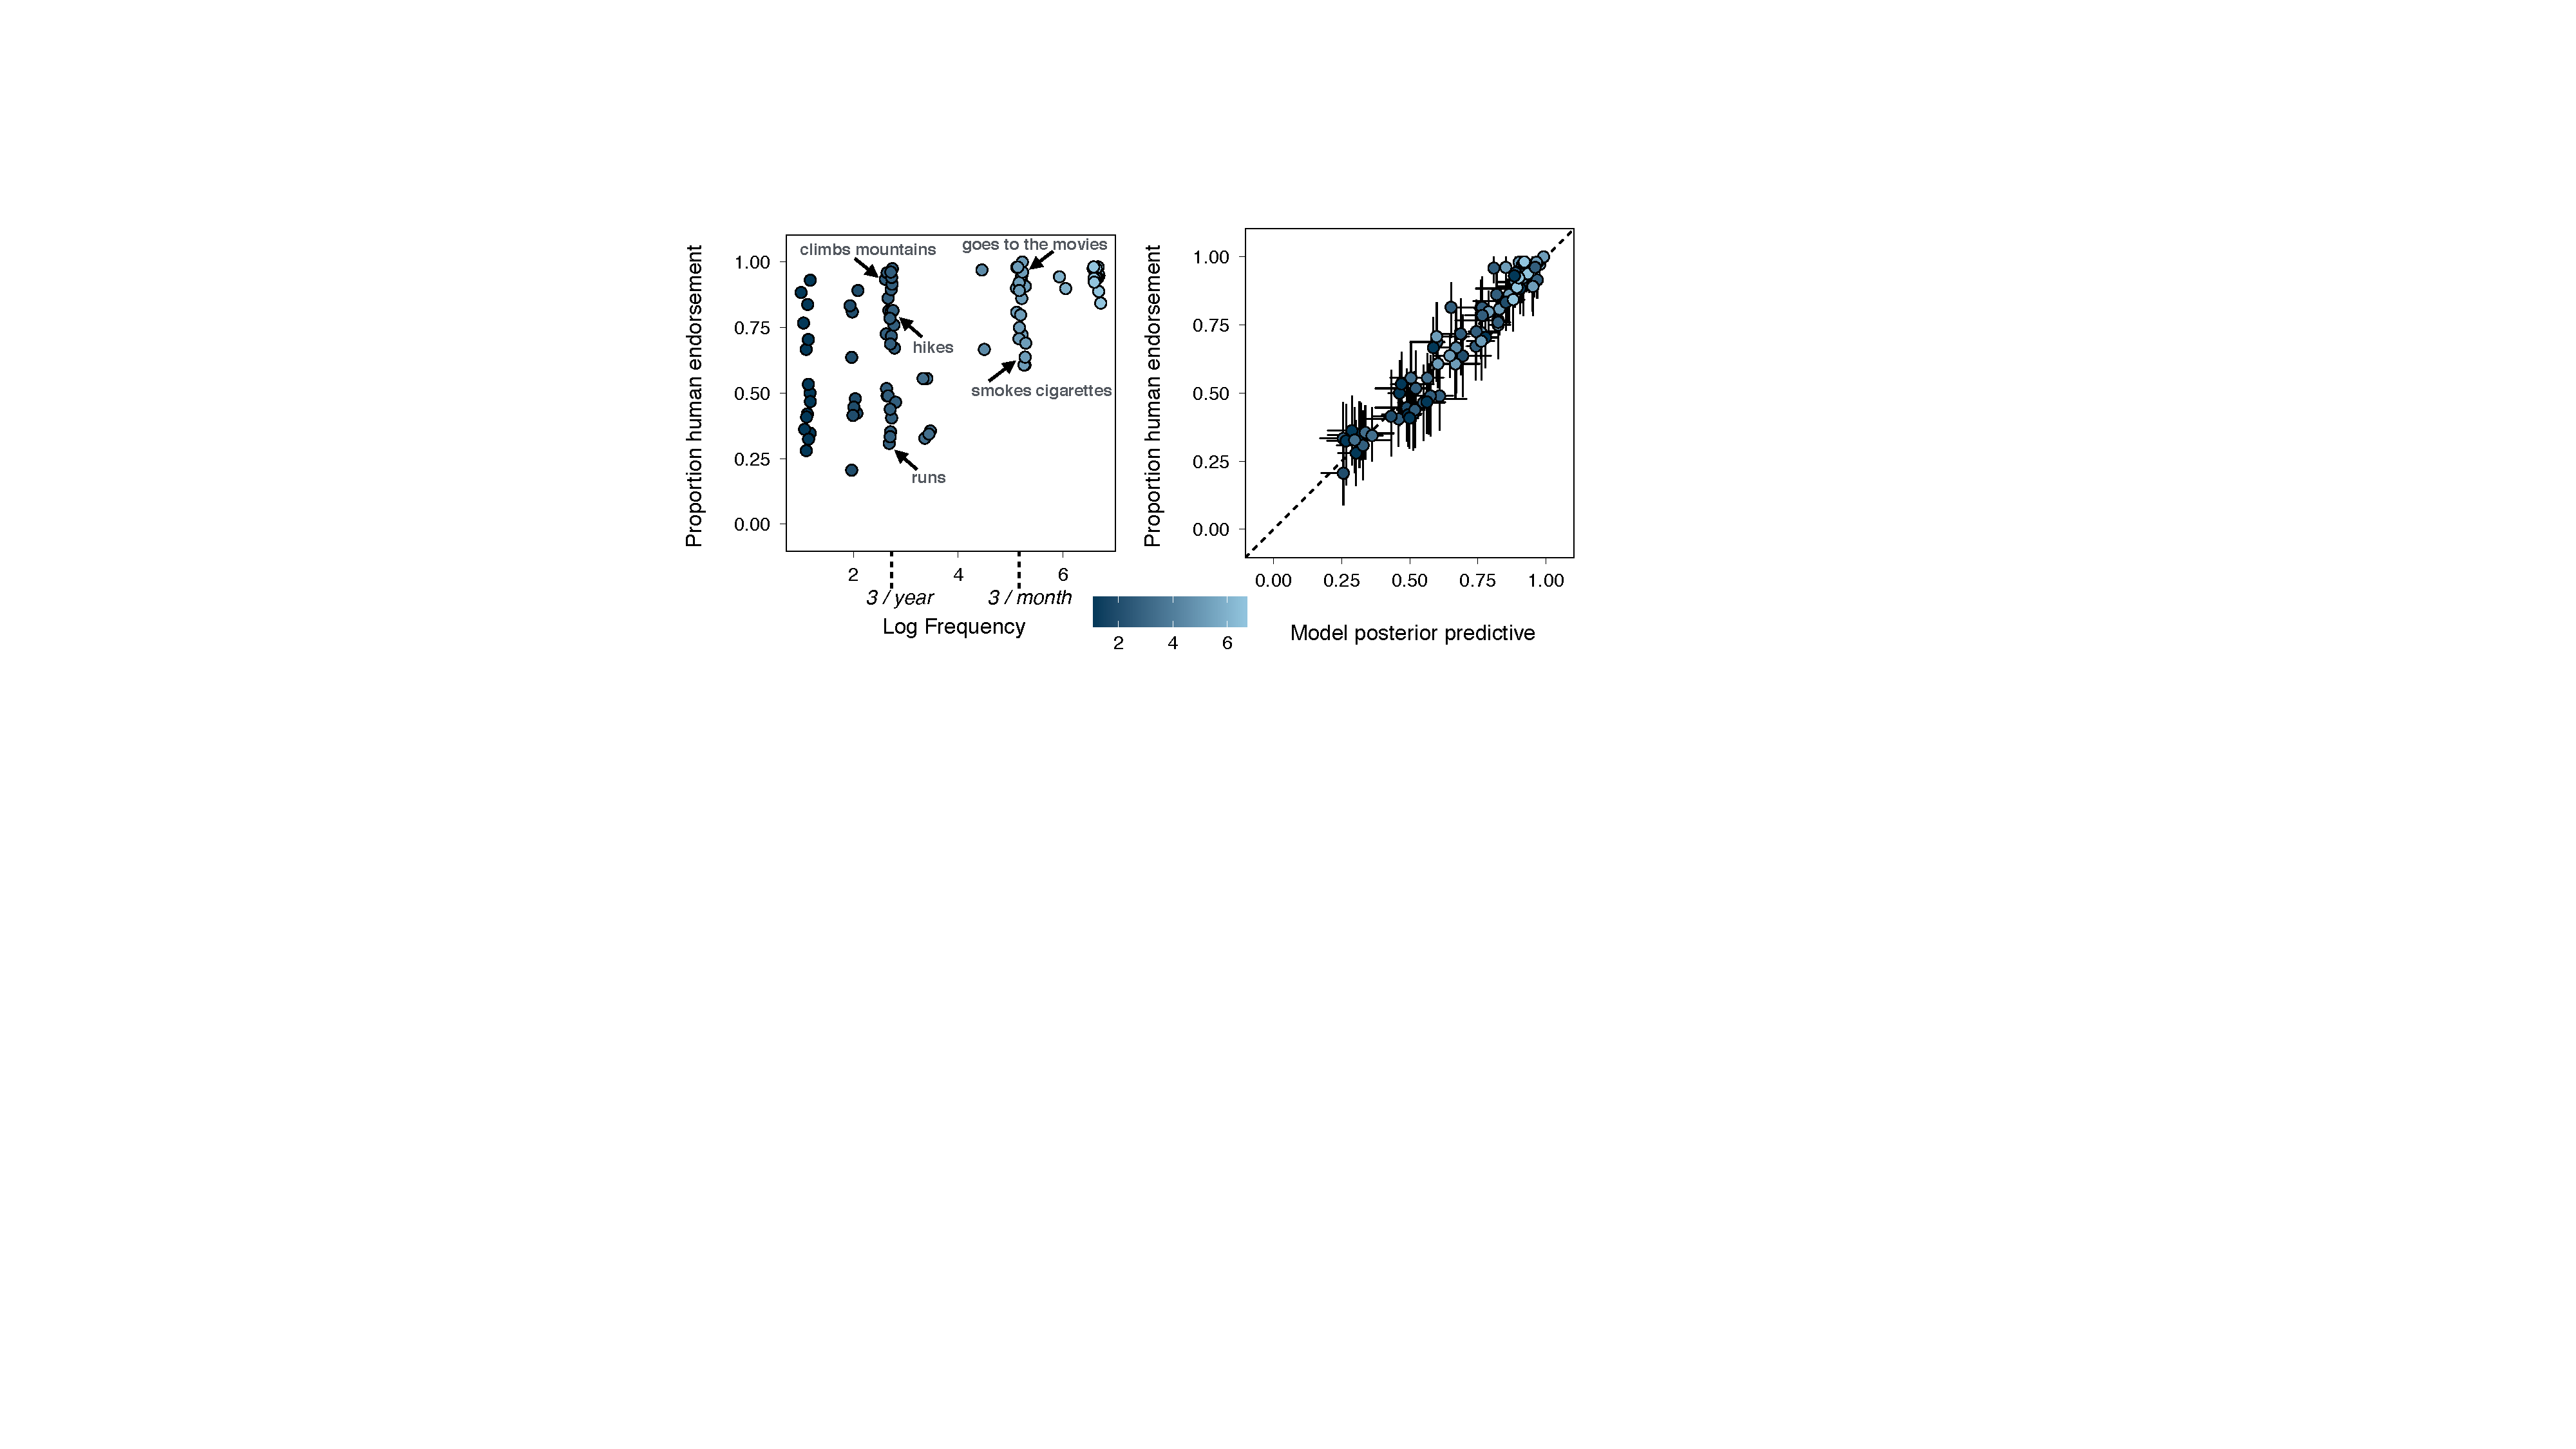
\includegraphics[width=0.84\textwidth]{tj-scatters-3}
  \caption{
  Human acceptability judgments as a function of the log frequency of action (left) and speaker $S_2$ model predictions (right) for ninety-three unique items (event \textsc{x} frequency). 
  Color denotes target-individual frequency of action (log scale), with lighter colors indicating more frequent actions. 
  Actual frequency noted on x-axis for examples (left).
  Error bars correspond to 95\% bootstrapped confidence intervals for the participant data and 95\% Bayesian credible intervals for the model predictions. 
  Error bars suppressed and points jittered on left facet for visual clarity.
  }
  \label{fig:tjScatters}
\end{figure*}

\vspace{-0.5ex}

\subsection{Data analysis and results}
We built a Bayesian data analysis model for this prior elicitation task.
Question 1 elicits the proportion of people who have done an action before. 
We model this data as coming from a Beta distribution: $d_{1} \sim \text{Beta}(\gamma_{1}, \xi_{1})$. 
Question 2 elicits the rate, or relative frequency, with which a person does the action.
This was modeled by a log-normal distribution: $\ln d_{2} \sim \text{Gaussian}(\mu_{2}, \sigma_{2})$. 
Each item was modeled independently for each gender.
%%
%\begin{minipage}{0.5 \textwidth} \small
%\begin{align*}
%d_{1} &\sim \text{Beta}(\gamma_{1}, \xi_{1}) \\
%\ln d_{2} &\sim \text{Gaussian}(\mu_{2}, \sigma_{2}) \\
%\end{align*}
%\end{minipage}
%%
We implemented this model using the probabilistic programming language WebPPL \cite{dippl}, and found the credible values of the parameters by running MCMC for 100,000 iterations, discarding the first 50,000 for burnin.
%
%The parametrized priors are a reasonable description of the prior elicitation data, though 

The priors elicited cover a range of possible parameter values as intended (Figure \ref{fig:priorScatter}, scatter), resulting in parametrized distributions of dramatically different shapes (insets).  
We observe a correlation in our items between the mean \% of Americans who have \textsc{done action} before (Question 1) and the mean log-frequency  of action (Question 2) ($r_{1,2} = 0.74$).
Items that tend to be more popular actions also tend to be more frequent actions (e.g. \emph{wears socks}) and visa-versa (e.g. \emph{steals cars}), though there are notable exceptions (e.g. \emph{plays the banjo} is not popular but done frequently when done at all, as is \emph{smokes cigarettes}; \emph{goes to the movies} is a popular activity though not done very often). 
This diversity is relevant because the speaker model (Eq.~\ref{eq:S2}) will produce habitual sentences (e.g. \emph{Sam goes to the movies vs. the ballet.}) contingent on the shape of the prior distribution. 

From the inferred parameters and assumed functional forms, we get an inferred $P(\lambda)$ modeled as a mixture of individuals with the possibility of carrying out the action and those without the possibility of doing it. 
That is, $P(\lambda)$ was constructed by sampling $\lambda$ as follows:
%That is, the posterior predictive of the prior data was constructed by forward-sampling the mixture component $\theta$ (determined by Q1: number of people who had done the action before, see Expt.~1 data analysis); if the sampled person was the kind of person to have done the action before, the frequency was sampled a likely frequency of action (determined by Q2); if they were not the type of person to have done the action, we assume they will never or only rarely do it. \ndg{never or rarely??}
%\begin{minipage}{0.5 \textwidth} \small
\begin{align}
\theta & \sim \text{Beta}(\gamma_{1}, \xi_{1}) \nonumber \\ 
\ln \lambda & \sim \begin{cases}
		\text{Gaussian}(\mu_{2}, \sigma_{2}) &\mbox{if } \text{Bernoulli}(\theta) = \textsc{t} \label{eq:priorModel}  \\
				\delta_{\lambda=-\infty} &\mbox{if } \text{Bernoulli}(\theta) = \textsc{f} \\
		\end{cases}
\end{align}
%\end{minipage}
In addition to specifying the correct way to combine our two prior-elicitation questions, using this inferred prior in our language model resolves two technical difficulties: (1) It smooths effects that are clearly results of the response format\footnote{For example, a very common rating is \emph{1 time per year}. Presumably participants would be just as happy reporting \emph{approximately} 1 time per year; the raw data does not reflect this due to demands of the dependent measure.} 
and (2) it better captures the tails of the prior distribution which have relatively little data and need to be regularized by the analysis.
Figure \ref{fig:priorScatter} (right) shows example inferred priors.
%, which receive such low probability to require many more participants in order to sample accurately.

Some items show substantial differences between the genders (e.g. \emph{wears a bra}) and some show subtle differences (e.g. \emph{watches professional football}). 
%It is \emph{a priori} unclear whether or not $P(x)$ in Eqs.~\ref{eq:L1}, \ref{eq:L0} is the distribution over frequency of action with respect to \emph{all people}, or if it is restricted to be gender specific.
%For example, are the frequency conditions by which a man would qualify to ``wear a bra'' (habitually) different than those by which a woman would qualify to ``wear a bra''?
We will explore the possibility of different truth conditions for habituals of different gendered characters in Experiment 2, for select items with priors that differ substantially by gender.
%In order to explore this possibility, we will select items with priors that differ by gender to explore more closely in Experiment 2.


%\mht{I've cut out the "posterior predictive" $r^2$ because I think it is not a reasonable metric. We should really come up with an appropriate fitness metric.}

%To assess how well these parametrized priors capture the prior elicitation data, we compare the posterior predictive distribution to the experimental data.
%We do this by discretizing the distributions as well as truncating at the endpoints 
%The posterior predictive distributions reconstruct the experimental data reasonably well for both question 1 ($r^2_{1} = 0.86$) and question 2 ($r^2_{2} = 0.68$) \mht{are there systemic deviations?}, and we use these parameterized priors going forward.

%\ndg{talk about gender differences?}

\section{Experiment 2: Felicity judgments}
A present-tense habitual sentence is of the form \textsc{singular noun phrase} $+$ \textsc{present tense simple verb phrase} (e.g. \emph{Bill smokes cigarettes.}).  
We next explore the endorsements of habituals of this form made from the items whose propensity priors were measured in Experiment 1. 
%\ndg{specifcy the grammar of the habitual constructions used more precisely (got / gets).. a singular noun (proper noun? person name?) combined with a present simple verb phrase??}

\subsection{Methods}

%\subsubsection{Participants}
\noindent {\bf Participants}
We recruited 150 participants from MTurk. %\footnote{
To arrive at this number, we performed a Bayesian precision analysis to determine the minimum sample size necessary to reliably ensure 95\% posterior credible intervals no larger than 0.3 for a parameter whose true value is 0.5 and for which the data is a 2 alternative forced choice. This analysis revealed a minimum sample size of 50 per item; since participants only completed about one third of the items, we recruited 150 participants.
%}
The experiment took 4 minutes on average and participants were compensated \$0.55 for their work.

%\subsubsection{Procedure and materials}
\noindent {\bf Procedure and materials}
On each trial, participants were presented with a \emph{past frequency statement} for a given event of the form: ``In the past M \{weeks, months, years\}, \textsc{person} \textsc{did x} 3 times''.
For example, \emph{In the past month, Bill smoked cigarettes 3 times}.
The particular intervals used (number M and window \{weeks, months, years\}) were selected after examining the predictions of the speaker model (Eq.~\ref{eq:S2}), for each item independently, to yield a variety of predicted endorsement rates.
The items were the same as in Expt. ~1.

Participants were asked whether they agreed or disagreed with the corresponding habitual sentence: ``\textsc{person does x}'' (e.g. \emph{Bill smokes cigarettes}).
Participants saw 25 out of the 31 items paired randomly with a male or female character name; the other 6 trials were presented with both male and female names (on separate trials; 37 trials total) to explore the nature of the contrast class (see Model section). 
%These 6 items were chosen because the priors for men and women varied substantially in Expt.~1; this will allow us to explore whether or not the prior distribution in Eq.~\ref{eq:L1}, \ref{eq:L0} should be with respect to all people or to males and females separately. 
%(e.g. if there is a frequency at which a male would be judged to (habitually) \textsc{wear a bra} but a woman would not be judged to). 
%\ndg{unclear what we did with these six items. the way it's phrased makes it sound like we only collected data for these 6...}
The experiment in full can be viewed at \url{http://stanford.edu/~mtessler/habituals/experiments/truth-judgments/tj-2.html}.

%The model predicts that some items would not exhibit variability in endorsements in given ranges (e.g. if a person stole a car 3 times in the past \emph{week} vs. \emph{month}); we omitted particular intervals when the model predicted non-meaningful differences in endorsements. 

%\subsubsection{Materials}

%\subsection{Behavioral results}
\subsection{Results}
\noindent {\bf Behavioral results}
On each trial of the experiment, the participant was told a person did a particular action 3 times during some time window. 
Figure \ref{fig:tjScatters} (left) shows the correspondence between the frequency of the event (normalizing to a 5-year time scale and taking the logarithm) and the felicity of the corresponding habitual sentence. 
It is clear that a habitual sentence can receive strong agreement even when the actions are very infrequent (log frequency $\sim$ 1; 3 times in a 5-year interval; e.g. \emph{writes novels}, \emph{steals cars}).
We also see even when actions are done relatively frequently (e.g. 3 times in a one month interval; log frequency $\sim$ 5), there are habitual sentences participants are reluctant to endorse completely (e.g. \emph{wears socks}, \emph{drinks coffee}). 
In our data, actions completed with a high frequency (3 times in a one week interval; log frequency $\sim$ 6.5) receive at least 75\% endorsement, though there is still variability among them (e.g. between 10-25\% of people disagree with \emph{wears a watch} and \emph{wears a bra}). %, suggesting that even actions that are completed almost everyday can insufficient to generalize.
Overall, frequency of action predicts only a fraction of the variability in responses ($r^2(93) = 0.33$).
For actions that are done on the time scale of years or longer (lower median of frequency), frequency itself no longer explains the endorsements ($r^2(50) = 0.07$)

We further examined the six items for which we observed gender differences in the prior elicitation task (Expt.~1).
We find no differences between endorsements of the habitual of characters with male and female names, and overall, the mean endorsements by gender are strongly correlated $r(93) = 0.91$. 
This may be because the felicity of habitual sentences depends on a comparison to individuals of both genders (i.e, the \emph{contrast class} is other people; not just other men or women). 
Less interestingly, the lack of a difference may be the result of gender being not very salient in our paradigm, perhaps because the names used were not sufficiently gendered.
%It is conceivable that elicit gender-differences in truth conditions could be elicited if the gender-specific contrast is made salient (e.g., by making salient stereotypes) .
% It is transparent to the participant that we are changing the frequencies and the actions, and perhaps less salient that the gender of the character is changing. 

%\mht{compare with split half correlation?}
%\ndg{say something more about why this is? or save this for model comparison? what does model predict?}

%We observe that none of our items receive less than 25\% endorsement (i.e. only 75\% of participants disagree with the felicity of the utterance).
%This may be due to the fact that actor has done the action in the past a plurality of times; we would expect to get strong disagreement with the habitual when the person has never done the action, or perhaps done it only once.


\begin{figure*}[t]
\centering
%  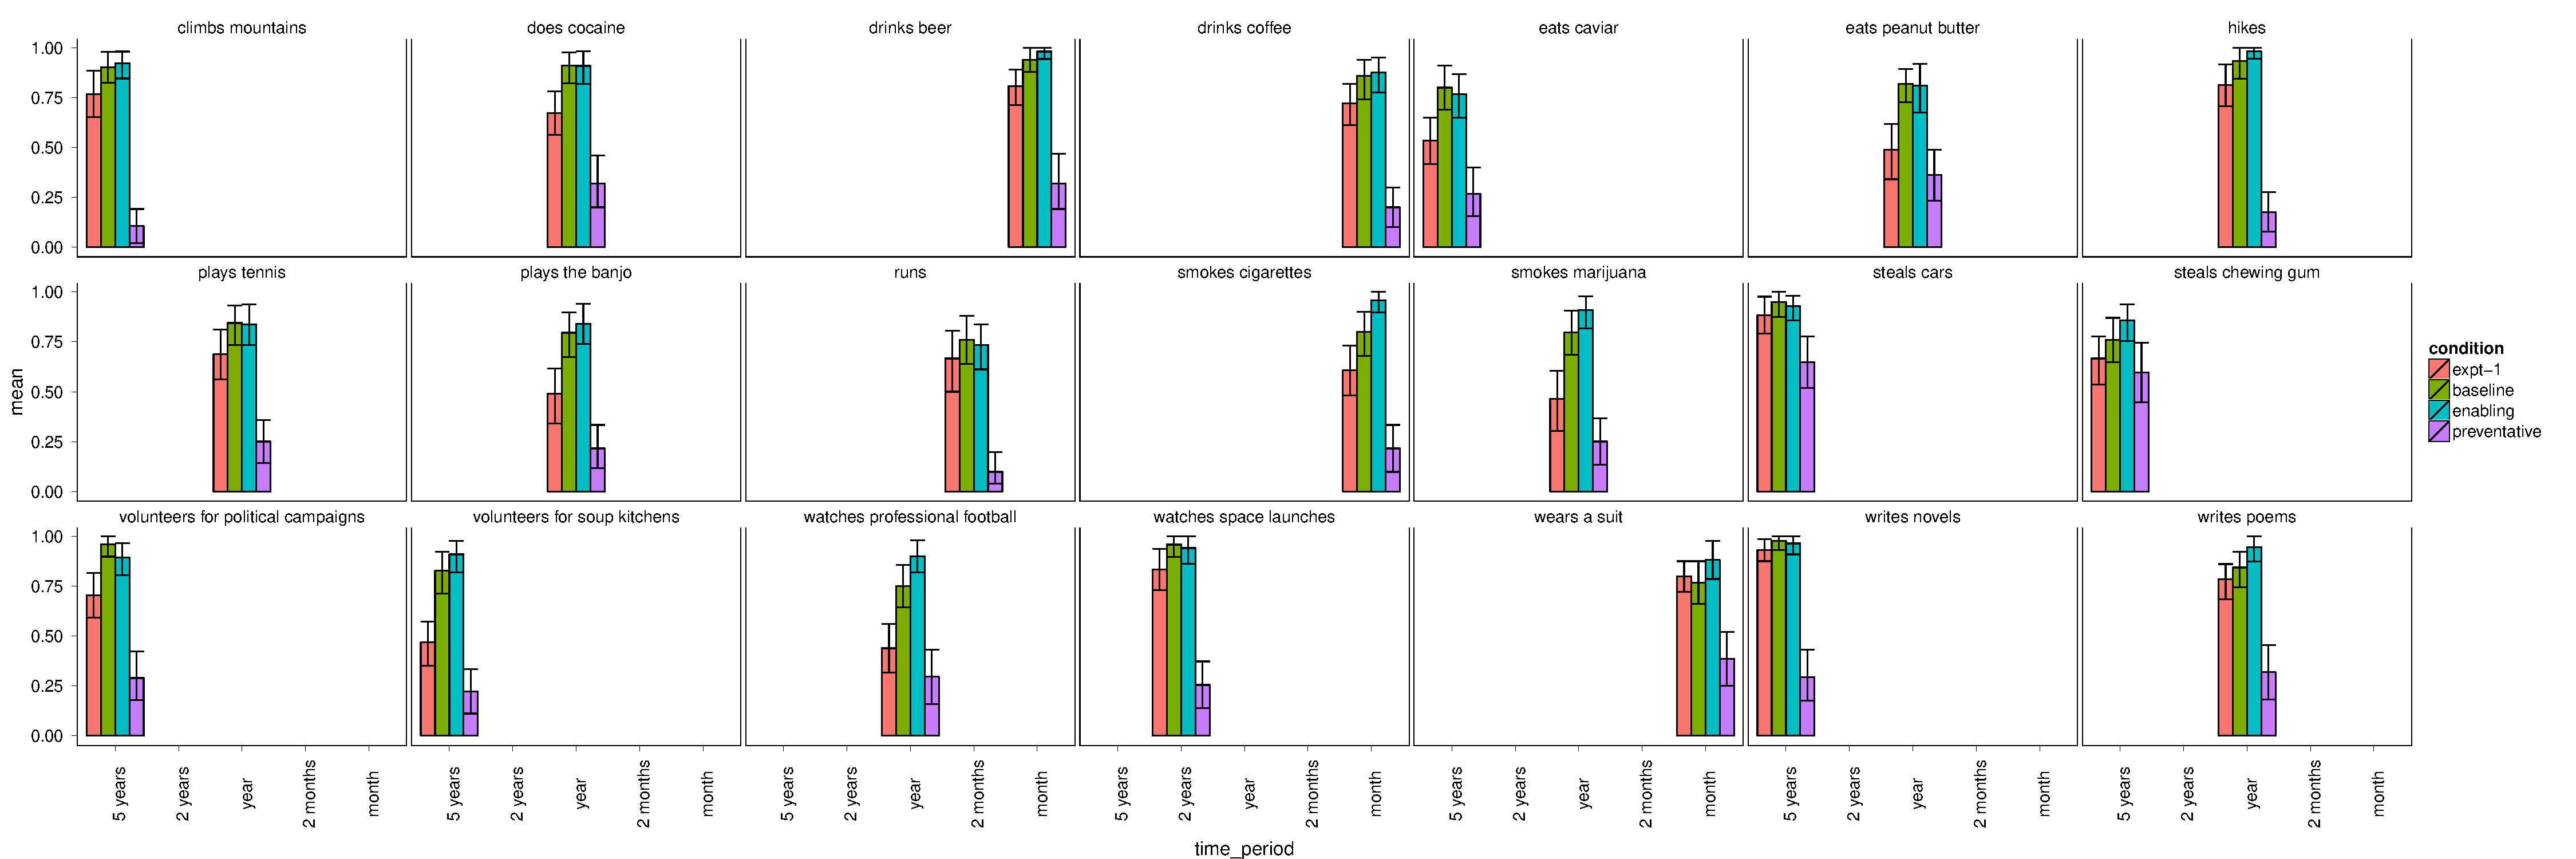
\includegraphics[width=\textwidth]{truth-judgments-3items-withtj2.pdf}
  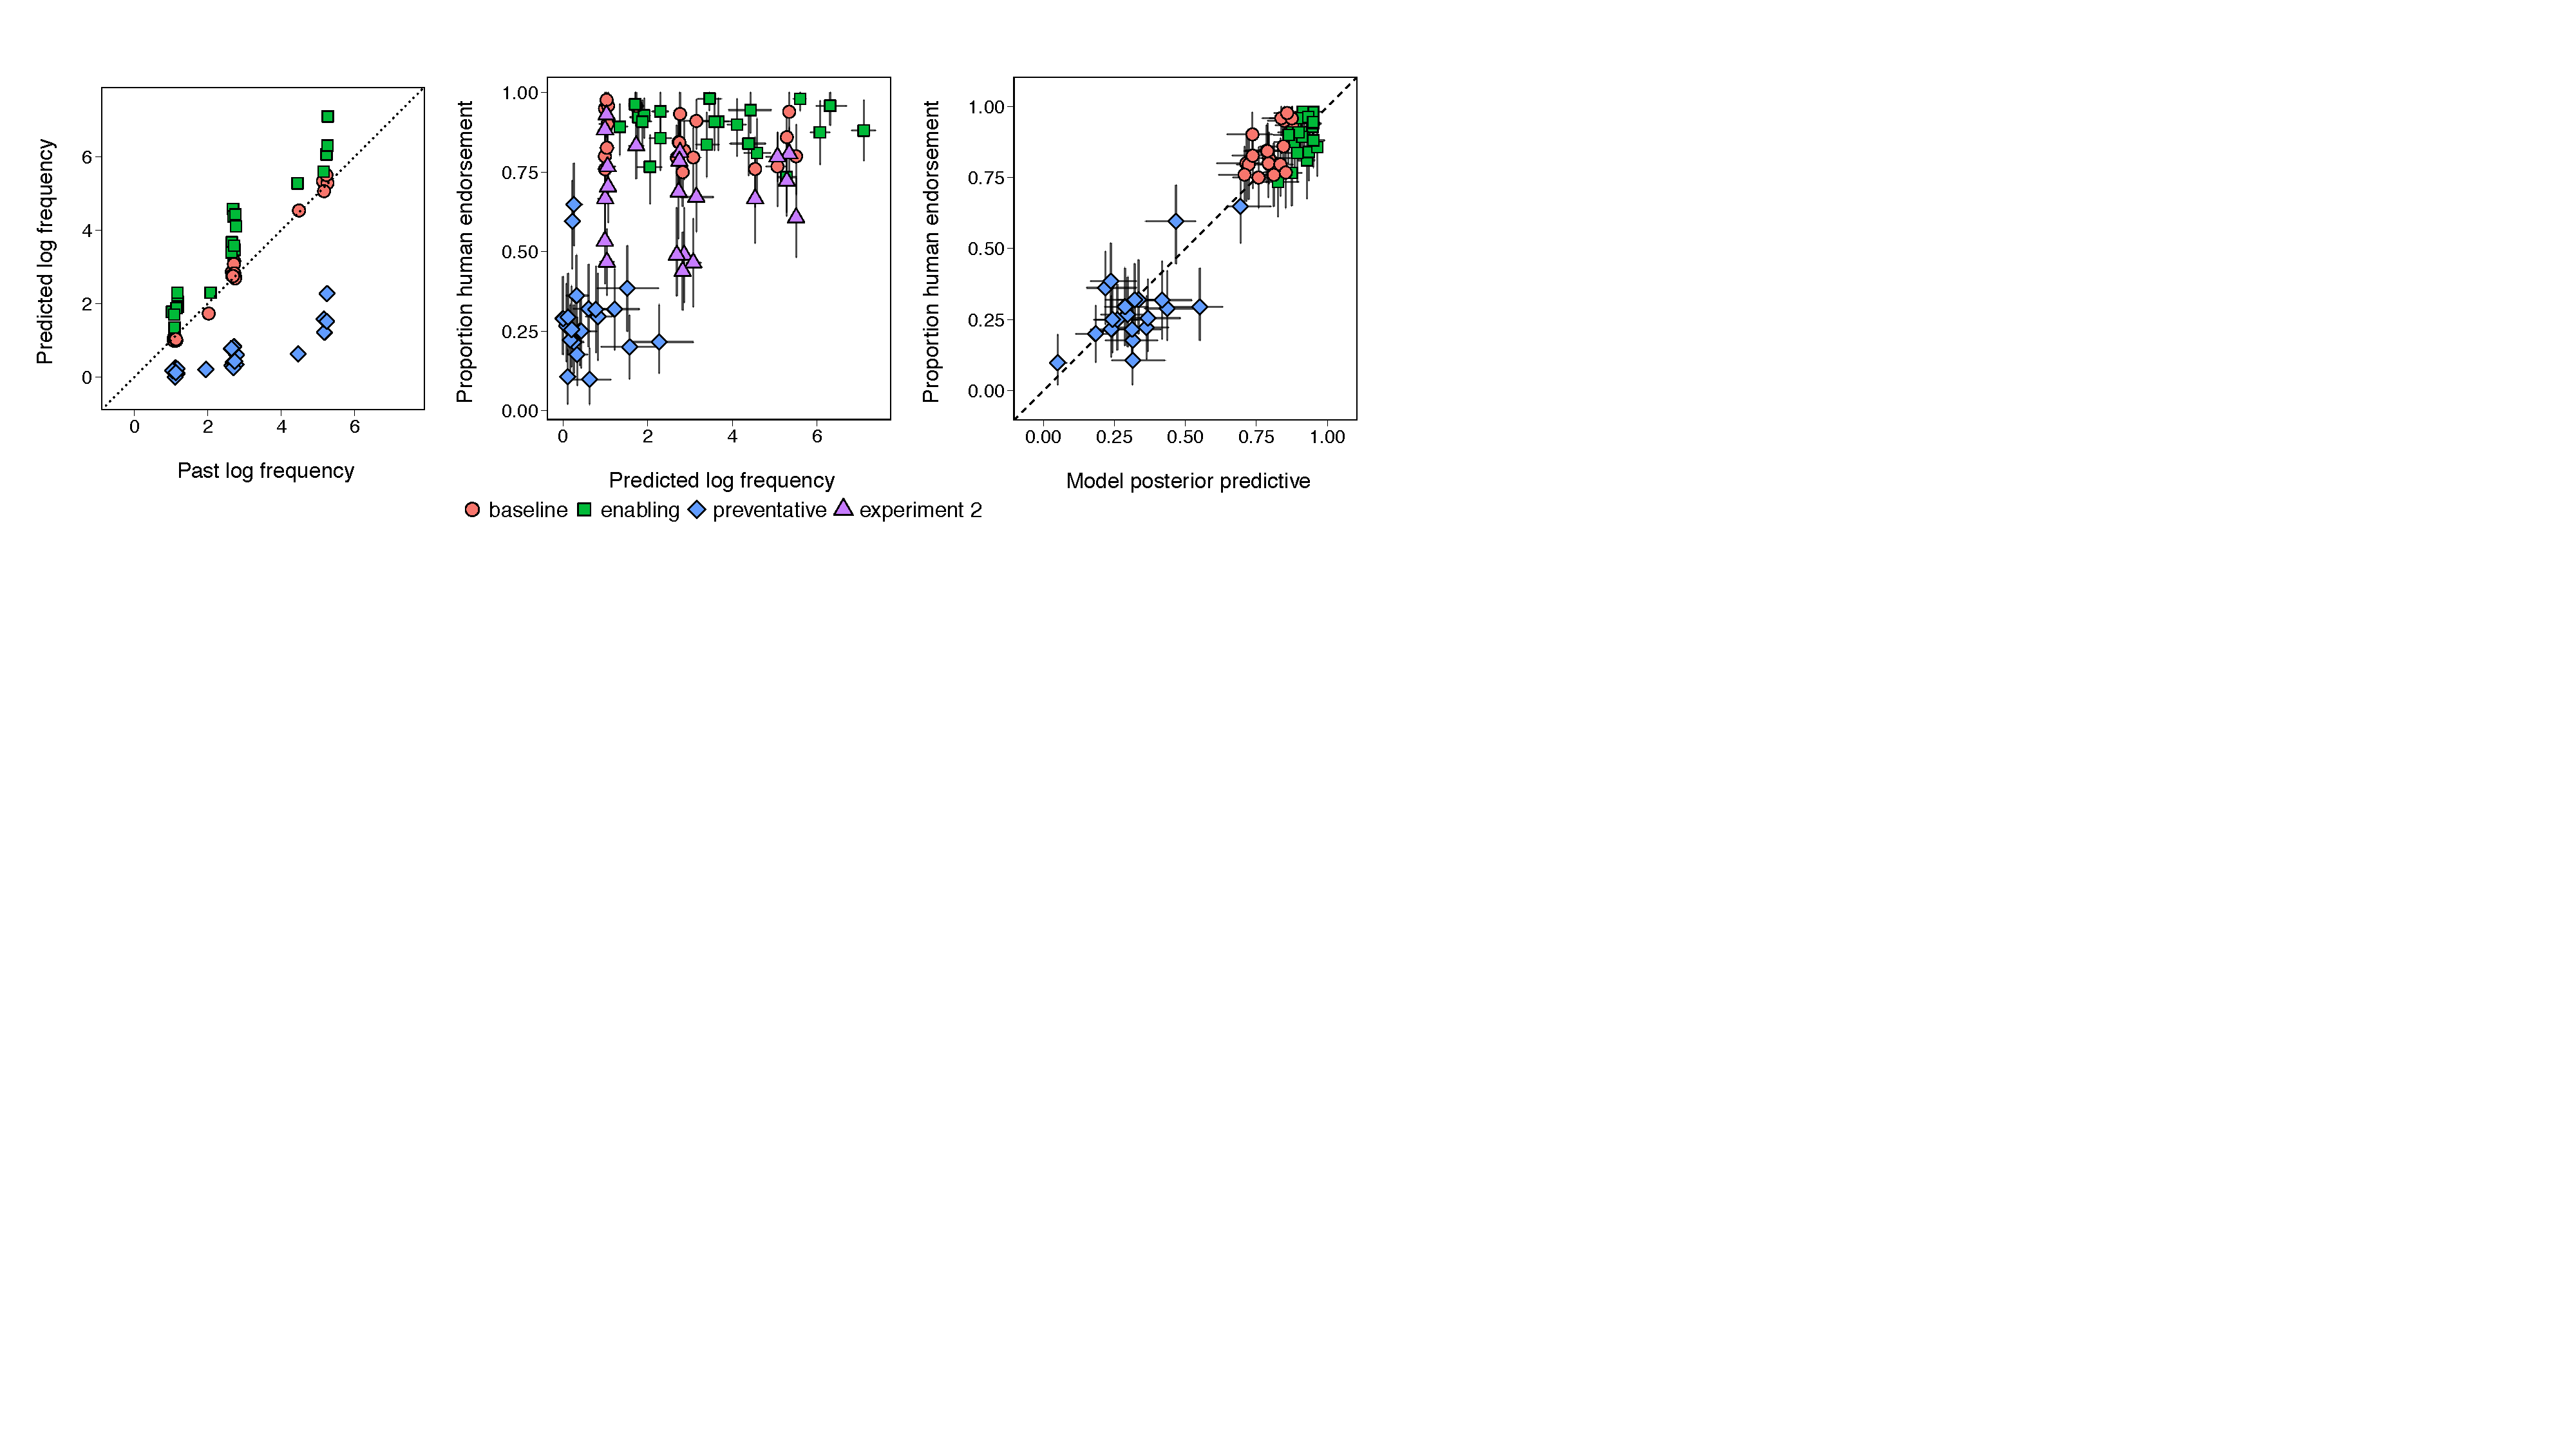
\includegraphics[width=\textwidth]{expt3-4-scatters-camera.pdf}
  \caption{Left: Predicted log frequency as a function of past log frequency given to the participant (Expt. 3a; CIs suppressed and jitter added for visual clarity).
  Middle: Human endorsements of habitual sentences (Expt. 3b) vs. Predicted log frequency (Expt. 3a), with data for corresponding items from Expt. 2 (assumed to have the same predictive log frequency as baseline). 
  Right: Endorsements (Expt. 3b) vs. Speaker $S_2$ model predictions using empirically elicited predictive frequencies (Expt. 3a).}
  \label{fig:tj3}
  \vspace{-7pt}
\end{figure*}

%\subsection{Model fit and results}
\noindent {\bf Model fit and results}
We used the pragmatic speaker model $S_2$ (Eq.~\ref{eq:S2}) with the priors elicited above (Expt.~1) to predict felicity judgments in Expt.~2, assuming the target propensity (to be conveyed by $S_2$) is the provided frequency.
Because we observe no difference between the felicity judgments for habituals of male and female characters, we use a 50\% mixture of the inferred priors for each gender to construct a single frequency distribution $P(\lambda)$ across individuals.
The model has two free parameters---the speaker optimality parameters, $\alpha_i$, in Eqs.~\ref{eq:S2} \& \ref{eq:S1}. 
%Additionally, we include a data analytic parameter to model random guessing behavior; this provides a rough measure of how much variance is unexplained by the pragmatics model. 
We use Bayesian data analytic techniques to integrate over these parameters \cite{LW2014}, comparing the posterior predictive distribution to the empirical data in Expt.~2.
%To attain credible values of the model parameters as well as 
To construct the posterior predictive distribution over responses, we collected 2 MCMC chains of 100,000 iterations, discarding the first 50,000 iterations for burn in.
The Maximum A-Posteriori value and 95\% highest probability density interval for $\alpha_1$ is 19.3 [14.9,19.9] and $\alpha_2$ is 1.5 [1.4,1.6].
%The MAP and HPD interval for the data-analytic guessing parameter is 0.004 [0.0003, 0.03], suggesting that there is not a substantial amount of the data that is better explained by a model of random guessing than by our pragmatic speaker model.

As shown in Figure \ref{fig:tjScatters}, right, the probabilistic pragmatics model does a good job of accounting for the variability in responses ($r^2(93) = 0.94$), including actions done on the time scale of years or more  ($r^2(50) = 0.92$).
The model decides when the habitual is a useful way to describe the person's behavior, assuming that what the person did in the past is representative. 
This raises an interesting question: Does the propensity communicated by the habitual indicate an objective, past frequency or a subjective, future expectation?


\section{Experiment 3: Objective frequency versus subjective expectation}



%People change in a way that natural kinds cannot: People can modify their behavior overnight.
%Yet, there is an ambiguity in the frequency degree semantics over which the pragmatic theory operates.
%In some sense, one can only know \emph{past frequency} of action because that is all that has occurred.
%On the other hand, language has a communicative function, and only \emph{predictive frequency} will be helpful in the future.

While past frequency is often a good indicator of future tendency, people can change abruptly due to a variety of decisions and outside events.
Does habitual language communicate propensity in terms of past frequency or future expectations?
In this set of experiments, we address this by introducing causal factors that enable or prevent future actions (e.g. buying cigarettes; developing an allergy).
In Expt.~3a, we measure \emph{predictive frequency} when past frequency alone is observed and when these causal factors are introduced.
In Expt.~3b, we examine felicity judgments of the habitual sentence (e.g. \emph{John smokes cigarettes.}; \emph{John eats peanut butter.}) in the presence of these causal modifiers.
This will allow us to test whether habituals are best explained by a speaker $S_2$ who communicates the known past or expected future frequency.
% and use the speaker $S_2$ model to predict the truth judgments using the elicited \emph{predictive frequency}  as the input to the model.
%\ndg{pose the question of this expriment more clearly: is propensity about past frequency or future expectations? then say briefly how we address it.}
%\vspace{-1.0ex}

\subsection{Experiment 3a: Prediction elicitation}
%\vspace{-1.0ex}

%\subsubsection{Method}
%\subsubsection{Participants} 

\noindent {\bf Methods}
We recruited 120 participants from MTurk, using the same criterion as Expt.~2.
The experiment took 4 minutes on average and participants were compensated \$0.40.

%\subsubsection{Procedure and materials}
%\noindent {\bf Procedure and materials}
The procedure was identical to Expt.~2 except for the inclusion of a second sentence on a subset of trials and the use of a different dependent measure. 
On all trials, participants were presented with a \emph{past frequency sentence} (see Expt.~2).
Additionally, on one third of the trials, participants were presented with a \textbf{preventative sentence} (e.g. \emph{Yesterday, Bill quit smoking.}). %that aimed to decrease the 
On one third of the trials, participants were presented with an \textbf{enabling sentence} (\emph{Yesterday, Bill bought a pack of cigarettes.}) %that sought to reinforce the past frequency that aimed to increase the acceptability of the habitual sentence when the past frequency evidence was not strong. 
The final third of trials had no additional evidence and were identical to Expt.~2. 

Only twenty-one of the original thirty-one items were used in order to shorten the experiment.
To increase expected variability, participants saw only the frequencies that led to most intermediate endorsement of the habitual in Expt.~2. 
In addition, we did not include separate trials for both male and female names for the select items we did in Expt.~2, since we saw no differences in their endorsements of the habitual.
%The dependent measure was the same as in Expt.~2. 

%The only difference from Expt.~3 is in the dependent measure.
Participants were asked ``In the next \textsc{time window}, how many times do you think \textsc{person} does \textsc{event}?'', where the \textsc{time window} was the same as given in the \emph{past frequency statement}.
The experiment in full can be viewed at \url{http://stanford.edu/~mtessler/habituals/experiments/priors/predictive-1.html}.


%\vspace{-1.0ex}
\subsection{Behavioral results}

Figure \ref{fig:tj3} (left) shows the predicted future frequency as a function of the past frequency given to the participant and the type of causal information given. 
We observe in the baseline condition that future frequency perfectly tracks past frequency (e.g. participants believe if a person smoked cigarettes 3 times last month, they will smoke cigarettes 3 times next month). 
This means that our model makes identical predictions for Expt.~2 whether the target is past frequency or expected future frequency (indicating, as expected, that we must look to the new data to distinguish these models).
% the assumption we used in our model of Expt.~2, where the speaker model intended to communicate past frequency.
%; testing the correspondence of past frequency with future frequency allows us validate the model predictions in Expt.~2 (where past frequency was assumed to be the target of communication).
Critically, we observe the preventative information appreciably decreasing and the enabling information slightly increasing predicted frequency (Figure \ref{fig:tj3} left; blue and green dots).




\subsection{Experiment 3b: Felicity judgments}


%\subsubsection{Method}
%\subsubsection{Participants} 

\noindent {\bf Methods}
We recruited 150 participants from MTurk, using the same criterion as Expt.~2.
The experiment took 4 minutes on average on participants were compensated \$0.40 for their work.
None of the participants had completed Expt.~3a.
%\subsubsection{Procedure and materials}
The only difference from Expt.~3a is the dependent measure. 
On each trial, participants were asked if they agreed or disagreed with the corresponding habitual sentence (as in Expt.~2).
The experiment in full can be viewed at \url{http://stanford.edu/~mtessler/habituals/experiments/truth-judgments/tj-3-preventative.html}.
%The experiment in full can be viewed at \url{http://stanford.edu/~mtessler/habituals/experiments/truth-judgments/tj-3-preventative.html}.


%\vspace{-1.0ex}
\subsection{Results}
%\vspace{-0.5ex}

There is a clear and consistent negative effect of preventative information on endorsements for the habitual sentence (Figure \ref{fig:tj3}, middle; blue points).
When collapsing across items and subjecting the data to a generalized mixed-effects model with random by-participant effects of intercept and random by-item effects of intercept and conditions, we find evidence for a small effect of \emph{enabling} conditions on endorsements (M =  0.89; 95\% Bootstrapped CI [0.88, 0.91]) as compared to baseline (M = 0.85 [0.83, 0.87]) [$\beta = 0.42; SE = 0.15; z = 2.8$]%; p = 0.005$]
, and a large effect of \emph{preventative} conditions on endorsements (M = 0.29 [0.26, 0.31]) [$ \beta = -3.22; SE = 0.21; z = -15.2$].%; p < 0.001$]. 
%\mht{should I add points from Expt. 2 to left-most scatter, or maybe there is a better plot?}

We use the mean predicted log frequency from Expt.~3a as the input to the speaker $S_2$ model to predict the felicity judgments measured in Expt.~3b.
We infer the one model parameter using the same analysis approach in Expt.~2. 
The model matches the data well ($r^2(63) = 0.91$; Figure \ref{fig:tj3}, right).
The same model using the past frequency as the object of communication does not match the data at all ($r^2(63) = 0.02$).
These results suggest that the felicity of habituals is based on an underlying scale of predicted future propensity, not merely the observed frequency in the past.

Interestingly, we observe endorsements in this experiment that are appreciably higher than in Expt.~2 for the same items (Figure \ref{fig:tj3}, middle; red vs. purple points). 
This may be due, in part, to an effect of the experimental context on participants: 
in this experiment the overall population of frequencies is much lower (both because we selected moderate frequencies from Expt.~2 and because of the preventative information) and participants may infer that the experimenter believes this to be a representative range and adjust judgments accordingly. Future investigation into this issue is warranted.

%Participants are viewing extra information that strongly disables the action from occurring in may cases; when that information is not present, participants may be more inclined to endorse the habitual.
%This may the be result of an inferential process about the experimenter's beliefs by the participant: Because the distribution of frequencies in this task was more limited than those used in Expt.~2, the participant may infer that the experimenter believes this to be a representative range and adjust her judgments accordingly.
%Future investigation into this issue is warranted.
% the frequencies supplied in the task
%\ndg{we should think about where in the model this calibration effect would be seen. Overall it would be nice to tie this expt more to the model, even if in a relatively shallow way.}

%     condition      mean  ci_lower  ci_upper
%        (fctr)     (dbl)     (dbl)     (dbl)
%1     enabling 0.8942857 0.8752381 0.9133333
%2     baseline 0.8504762 0.8304762 0.8714524
%3 preventative 0.2885714 0.2628333 0.3161905


%Generalized linear mixed model fit by maximum likelihood (Laplace Approximation) ['glmerMod']
% Family: binomial  ( logit )
%Formula: response ~ condition + (1 | workerid) + (1 + condition | habitual)
%   Data: d
%
%     AIC      BIC   logLik deviance df.resid 
%  2684.2   2744.7  -1332.1   2664.2     3140 
%
%Scaled residuals: 
%    Min      1Q  Median      3Q     Max 
%-3.8931 -0.4064 -0.2551  0.4292  7.4117 
%
%Random effects:
% Groups   Name                  Variance Std.Dev. Corr       
% workerid (Intercept)           0.891215 0.9440              
% habitual (Intercept)           0.316971 0.5630              
%          conditionenabling     0.004135 0.0643    0.09      
%          conditionpreventative 0.561694 0.7495   -0.61  0.73
%Number of obs: 3150, groups:  workerid, 150; habitual, 21
%
%Fixed effects:
%                      Estimate Std. Error z value Pr(>|z|)    
%(Intercept)            -2.1220     0.1791 -11.848  < 2e-16 ***
%conditionenabling      -0.4190     0.1508  -2.779  0.00546 ** 
%conditionpreventative   3.2262     0.2125  15.181  < 2e-16 ***
%---

%\subsection{Model results}


%\vspace{-1.0ex}
\section{Discussion}
We presented a computational model for communicating generalizations about events.
The model decides if a habitual sentence is a pragmatically useful way to describe a person's behavior, taking into account the listener's prior beliefs about the action---how common it is and the likely frequency (measured in Expt.~1).
% --- and the basic conversational principles to be truthful and informative.
We validated this model by eliciting felicity judgments for habitual sentences covering diverse activities with a wide range of experimentally manipulated frequencies of action (Expt.~2).
We further investigated the nature of the underlying ``propensity'' scale by introducing enabling and disabling evidence, measuring the predicted future frequency (Expt.~3a) and using that, with the model, to predict the felicity of habitual sentences (Expt.~3b). 
To our knowledge, the experiments presented here are first empirical investigations into the truth conditions of habitual sentences and the first test of a formal model of habitual language.


%We use a formal theory of the semantics and pragmatics of habitual language in order to derive predictions about the felicity of habituals.
%We adopt as the underlying degree scale the \emph{propensity} with which a person does an action. 
%In Expts.~3 \& 4, we showed that the notion of propensity is tied to the future predictions. 
%Future predictions are important to communicate because the generalization is only useful if it helps predict future events. 
%It further suggests the underlying scale is a subjective one that integrates observed frequency with top-down biases from an intuitive theory.

The model we present here is almost identical to a model we have used to describe generic language \cite{TesslerUnderReview}.
The only difference is in the underlying scale: for generics, it is the \emph{prevalence} of the property; for habituals, the \emph{propensity} of the action. 
This provides a formal bridge between generalizations about categories (i.e. \emph{generics}) and generalizations about events (i.e. \emph{habituals}), a connection often noted in the linguistics literature \cite{Carlson1977, Carlson2005, Cohen1999}. 
Generics often use a bare plural (e.g. \emph{Bears like to eat ants.}) and don't lay claim to any well-defined set of individuals (many bears may not like to eat ants).
Habituals use the simple present tense (e.g. \emph{John smokes}) without any well-defined period of time (John may go many days without smoking). 
In both cases, a pragmatically inferred threshold on prevalence or propensity, respectively, explains the varying truth conditions of these kinds of sentences.
% the set of individuals or on the period of time, respectively. 
Scales, and scalar representations, provide a simple and general quantitative way to express truth conditions.
%In the psychological literature, habituals have received relatively little attention compared to \emph{generics}. 

%We explore generalizations about events using the domain of human behavior as it provides a well-defined domain of events with wide variability in frequency of occurrence.
%We have preliminary evidence from Expt.~2 that the prior over which the intended meaning is derived $P(\lambda)$ is with respect to individuals from both genders: Felicity judgments did not vary appreciably across the two genders, even when the $P_{gender}(\lambda)$ did. 
%This begins addresses one aspect of the \emph{contrast class} with respect to which generic or habitual meaning is computed. 
%In general, the issue of how a contrast class is derived remains mysterious but it is central to understanding how the meanings of vague bits of language arise.
%% with respect to events in general, and future work should address this. 
%%\ndg{this paragraph is weak... figure out what we want to say, or remove.}

%Though we validate this model using the speaker component $S_2$ for the evaluation of the felicity of habitual sentences, this model naturally extends to capture \emph{comprehension} of habitual language using the listener $L_1$ component.

Accurately predicting the environment is critical for survival and development.
Habituals convey generalizations about events and are helpful for future predictions about events.
For example, knowing that an event generally happens may be a useful abstraction for causal inference \cite<e.g.>{Griffiths2005}.
Generalizations about people's behavior in particular---as we've investigated in this article---are important to understand, as they likely facilitate trait induction and essentialist beliefs \cite{Gelman1999}.
The computational model presented here provides a mathematical bridge between the way we talk about people's behavior and our intuitive theories of others and events.

% and may serve as the bridge between observations of particular instances in time and enduring, essentialist beliefs about people.
%\ndg{this paragraph should be revised to focus more on why habituals are important and how they fit into generalization and the mind more generally. mention traits only if this is relevant!}
%
%\ndg{note: in doing this revision it became clear to me that habituals are not about all kinds of event generalizations --- they are specifically about generalizing the tendency of an individual to be part of an event.... should make small adjustments to clarify this?}

%\mht{kind of rough and needs more flowers}
%
%Generics are ubiquitous in everyday conversation and in child-directed speech \cite{Gelman2008} and are thought to be central to how concepts are developed \cite{Gelman2004}.
%What might habitual language be used for?
%One possibility is that we describe individuals in terms of their enduring traits and habits. 
%Future work should explore this connection more directly.
%	
%\mht{kind of rough and needs more meat}
%The similarities between habitual and generic language may be useful for methodological reasons. 
%In Expt.~3, we manipulated participants' beliefs about the expected, future frequency of a behavior in a person.
%This showed that the underlying degree scale is likely to be \emph{predictive} frequency, as opposed to past frequency. 
%We were able to do this because people have rich, structured theories of people's behavior that varies over time. 
%In general, the different aspects of intuitive theories of people vs. categories may facilitate further exploration of how beliefs and language play off one another.


%The habitual sentences we explored were all presented in the simple, present tense.
%Generalizations can also occur in the past tense (e.g. \emph{Bill smoked}, or \emph{Bill used to smoke.}) and in the future tense (e.g. \emph{Bill will smoke}). 
%The present tense is interesting because it is \emph{a priori} unclear when, in time, the sentence is making reference to.  
%
%\begin{enumerate}
%\item Methodological implications (using habituals as opposed to generics)
%\item Contrast class finding (men vs women)
%\item Tense (past vs future vs present)
%\end{enumerate}


%people do things and infer what they \emph{are like} (e.g. if they often do this thing). 
%Understanding habitual language can shed light on a person's intuitive theories of other people, which might in turn be the basis of how we learn intuitive theories of groups (or, stereotypes). 
%Additionally, because of people's intuitive theories of others are so richly structured according to events (e.g. having hobbies, having a job, eating certain foods and not others; or more generally, being able to complete certain actions and not others),
%habitual language may give us insight into those theories. \red{eek}

%\vspace{-1.0ex}
\section{Acknowledgments}

This work was supported by NSF Graduate Research Fellowship DGE-114747 to MHT and a James S. McDonnell Foundation Scholar Award  and ONR Grant N00014-13-1-0788 to NDG.

%, by John S. McDonnell Foundation Scholar Award 220020252 
\bibliographystyle{apacite}

\setlength{\bibleftmargin}{.125in}
\setlength{\bibindent}{-\bibleftmargin}
\vspace{-1.5ex}

\bibliography{habituals-cogsci2016}


\end{document}
